\documentclass[11pt]{article}
\usepackage[margin=1in]{geometry}
\usepackage{amsmath,amssymb,amsthm,mathtools,bm}
\usepackage{graphicx,booktabs,subcaption}
\usepackage[hidelinks]{hyperref}
\usepackage{enumitem}
\allowdisplaybreaks

\newtheorem{proposition}{Proposition}[section]
\newtheorem{theorem}[proposition]{Theorem}
\newtheorem{remark}[proposition]{Remark}
\newtheorem{definition}[proposition]{Definition}

\newcommand{\R}{\mathbb{R}}
\newcommand{\E}{\mathbb{E}}
\newcommand{\Var}{\operatorname{Var}}
\newcommand{\Cov}{\operatorname{Cov}}
\newcommand{\diag}{\operatorname{diag}}
\newcommand{\Id}{I}
\newcommand{\trans}{\mathsf{T}}
\newcommand{\Ncal}{\mathcal{N}}
\newcommand{\norm}[1]{\left\lVert #1 \right\rVert}
\newcommand{\abs}[1]{\left| #1 \right|}
\newcommand{\Lap}{\operatorname{Laplace}}
\newcommand{\sgn}{\operatorname{sgn}}

\title{Laplace AR(1): the first non-Gaussian extension\\[2mm]
\large Local clean energy, nonlinear score, and state-dependent interactions}
\author{}
\date{}

\begin{document}
\maketitle

\begin{abstract}
We replace the Gaussian AR(1) innovations by Laplace innovations while keeping the same one-step recursion,
\[
 a_{k+1}=\alpha a_k+\eta_k,
 \qquad
 \eta_k\sim\Lap(0,b).
\]
To keep the exposition controlled we take $a_0\sim\Ncal(0,\sigma_0^2)$ independent of the innovations. The clean trajectory still has a local factorization,
\[
 p_0(a)
 =
 \frac{e^{-a_0^2/(2\sigma_0^2)}}{\sqrt{2\pi\sigma_0^2}}
 \prod_{k=0}^{K-1}\frac{1}{2b}
 \exp\!\left(-\frac{\abs{a_{k+1}-\alpha a_k}}{b}\right),
\]
so the underlying Markov structure is nearest-neighbor and explicit. After Ornstein--Uhlenbeck corruption,
\[
 x=e^{-t}a+\sqrt{1-e^{-2t}}\,z,
\]
the noisy density is smooth but no longer Gaussian. Its characteristic function is explicit and shows quartic and higher cumulants at every finite time. The score can nevertheless be written exactly in posterior-mean form,
\[
 S_t(x)=\nabla_x\log p_t(x)=-\frac{x-e^{-t}\E[a\mid x]}{\Delta_t},
\qquad \Delta_t=1-e^{-2t}.
\]
The Gaussian case is recovered only when the posterior mean is linear in $x$. Here it is not, so the score is nonlinear and is not determined by the covariance. A natural replacement for the constant Gaussian precision is the negative score Hessian
\[
 H_t(x):=-\nabla_x^2\log p_t(x)=\frac{1}{\Delta_t}\Id-\frac{e^{-2t}}{\Delta_t^2}\Cov(a\mid x),
\]
which is state-dependent. This note shows how Gaussianity, Markovianity, and locality separate once the innovations are non-Gaussian.
\end{abstract}

\section{Model and second moments}
We fix
\begin{equation}\label{eq:model}
 a_0\sim\Ncal(0,\sigma_0^2),
 \qquad
 a_{k+1}=\alpha a_k+\eta_k,
 \qquad
 \eta_k\stackrel{\text{i.i.d.}}{\sim}\Lap(0,b),
\end{equation}
with all random variables independent. The Laplace density and characteristic function are
\begin{equation}\label{eq:lap_pdf_cf}
\ell_b(u)=\frac{1}{2b}e^{-\abs{u}/b},
\qquad
\widehat\ell_b(q)=\E[e^{iq\eta}]=\frac{1}{1+b^2q^2}.
\end{equation}
The variance of one innovation is
\begin{equation}\label{eq:lap_var}
\Var(\eta_k)=2b^2.
\end{equation}

Although the law is non-Gaussian, the covariance recursion is exactly the same as in the Gaussian AR(1) model because only second moments are involved.
\begin{proposition}[Second moments]\label{prop:second_moments}
Let $\sigma_k^2:=\Var(a_k)$. Then
\begin{equation}\label{eq:var_laplace}
\sigma_k^2=\alpha^{2k}\sigma_0^2+2b^2\sum_{m=0}^{k-1}\alpha^{2m}.
\end{equation}
For $j\le k$,
\begin{equation}\label{eq:cov_laplace}
\Cov(a_j,a_k)=\alpha^{k-j}\sigma_j^2,
\qquad
\text{equivalently}
\qquad
\Cov(a_j,a_k)=\alpha^{\abs{j-k}}\sigma_{\min(j,k)}^2.
\end{equation}
\end{proposition}

\begin{proof}
Because $\eta_k$ is centered and independent of $a_k$,
\[
\sigma_{k+1}^2=\Var(\alpha a_k+\eta_k)=\alpha^2\sigma_k^2+2b^2.
\]
Iterating this recursion gives \eqref{eq:var_laplace}. For $j\le k$, unroll the recursion from time $j$ to time $k$:
\[
 a_k=\alpha^{k-j}a_j+\sum_{m=j}^{k-1}\alpha^{k-1-m}\eta_m.
\]
The second term is independent of $a_j$, hence
\[
\Cov(a_j,a_k)=\alpha^{k-j}\Var(a_j)=\alpha^{k-j}\sigma_j^2.
\]
Symmetry gives the second formula.
\end{proof}

Thus, if we compare to a Gaussian AR(1) model with innovation variance $\sigma_\eta^2=2b^2$, the two models have the same covariance. What changes is everything beyond the covariance.

\section{Clean joint density: local and explicit}
The map from $(a_0,\eta_0,\dots,\eta_{K-1})$ to $(a_0,a_1,\dots,a_K)$ is triangular with unit Jacobian because
\[
\eta_k=a_{k+1}-\alpha a_k.
\]
Therefore the clean joint density is obtained by direct substitution.
\begin{proposition}[Exact clean density]\label{prop:clean_density}
The clean Laplace AR(1) trajectory has density
\begin{equation}\label{eq:clean_density}
 p_0(a_0,\dots,a_K)
 =
 \frac{1}{\sqrt{2\pi\sigma_0^2}}e^{-a_0^2/(2\sigma_0^2)}
 \prod_{k=0}^{K-1}\frac{1}{2b}
 \exp\!\left(-\frac{\abs{a_{k+1}-\alpha a_k}}{b}\right).
\end{equation}
Equivalently,
\begin{equation}\label{eq:clean_energy}
-\log p_0(a)
=
\frac{a_0^2}{2\sigma_0^2}
+
\frac{1}{b}\sum_{k=0}^{K-1}\abs{a_{k+1}-\alpha a_k}
+\text{constant}.
\end{equation}
\end{proposition}

The clean energy is local: it is a sum of nearest-neighbor terms. Away from the residual hyperplanes $a_{k+1}-\alpha a_k=0$, the clean score exists and is also local.
\begin{proposition}[Clean score where differentiable]\label{prop:clean_score}
Assume $a_{k+1}-\alpha a_k\ne 0$ for all $k$. Then
\begin{align}
\partial_{a_0}\log p_0(a)
&=
-\frac{a_0}{\sigma_0^2}+\frac{\alpha}{b}\sgn(a_1-\alpha a_0), \label{eq:clean_score_0}\\
\partial_{a_k}\log p_0(a)
&=
\frac{\alpha}{b}\sgn(a_{k+1}-\alpha a_k)-\frac{1}{b}\sgn(a_k-\alpha a_{k-1}),
\qquad 1\le k\le K-1, \label{eq:clean_score_mid}\\
\partial_{a_K}\log p_0(a)
&=
-\frac{1}{b}\sgn(a_K-\alpha a_{K-1}). \label{eq:clean_score_K}
\end{align}
\end{proposition}

These formulas make the separation from the Gaussian case explicit:
\begin{itemize}[leftmargin=1.5em]
\item the clean interaction is still nearest-neighbor;
\item the clean score is now nonlinear and nonsmooth;
\item there is no constant precision matrix summarizing the model.
\end{itemize}

\section{Clean characteristic function}
Unrolling the recursion in \eqref{eq:model} gives, for each $k$,
\begin{equation}\label{eq:unroll}
 a_k=\alpha^k a_0+\sum_{m=0}^{k-1}\alpha^{k-1-m}\eta_m.
\end{equation}
Fix $s=(s_0,\dots,s_K)\in\R^N$. Then
\begin{align*}
\sum_{k=0}^{K}s_k a_k
&=
\left(\sum_{k=0}^{K}\alpha^k s_k\right)a_0
+
\sum_{m=0}^{K-1}\left(\sum_{k=m+1}^{K}\alpha^{k-1-m}s_k\right)\eta_m.
\end{align*}
Define the linear forms
\begin{equation}\label{eq:c_forms}
 c_0(s):=\sum_{k=0}^{K}\alpha^k s_k,
 \qquad
 c_{m+1}(s):=\sum_{k=m+1}^{K}\alpha^{k-1-m}s_k,
 \qquad m=0,\dots,K-1.
\end{equation}
Because $a_0,\eta_0,\dots,\eta_{K-1}$ are independent, the characteristic function factorizes.
\begin{proposition}[Exact clean characteristic function]\label{prop:cf_clean}
For $s\in\R^N$,
\begin{equation}\label{eq:cf_clean}
\varphi_0(s)
:=
\E\big[e^{i s^\trans a}\big]
=
\exp\!\left(-\frac12\sigma_0^2 c_0(s)^2\right)
\prod_{m=0}^{K-1}\frac{1}{1+b^2 c_{m+1}(s)^2}.
\end{equation}
\end{proposition}

\begin{proof}
Insert \eqref{eq:unroll} into $s^\trans a$ and use \eqref{eq:c_forms}:
\[
 s^\trans a=c_0(s)a_0+\sum_{m=0}^{K-1}c_{m+1}(s)\eta_m.
\]
Taking expectations and using independence gives
\[
\varphi_0(s)=\E[e^{ic_0(s)a_0}]\prod_{m=0}^{K-1}\E[e^{ic_{m+1}(s)\eta_m}].
\]
The Gaussian factor is $\exp(-\tfrac12\sigma_0^2 c_0(s)^2)$ and each Laplace factor is $(1+b^2c_{m+1}(s)^2)^{-1}$ by \eqref{eq:lap_pdf_cf}.
\end{proof}

\section{OU corruption: convolution and Fourier transform}
Let $z\sim\Ncal(0,\Id_N)$ independent of $a$, and define the noisy sample
\begin{equation}\label{eq:xt_def}
 x=e^{-t}a+\sqrt{\Delta_t}\,z,
 \qquad
 \Delta_t:=1-e^{-2t},
 \qquad
 \beta_t:=e^{-2t}.
\end{equation}
The noisy density is the Gaussian convolution
\begin{equation}\label{eq:conv}
 p_t(x)=\int_{\R^N}\phi_{\Delta_t}(x-e^{-t}a)\,p_0(a)\,da,
\end{equation}
where
\[
\phi_{\Delta_t}(y)=\frac{1}{(2\pi\Delta_t)^{N/2}}\exp\!\left(-\frac{\norm{y}^2}{2\Delta_t}\right).
\]
The characteristic function is even simpler.
\begin{proposition}[Exact noisy characteristic function]\label{prop:cf_noisy}
For every $s\in\R^N$,
\begin{equation}\label{eq:cf_noisy}
\varphi_t(s)
:=
\E[e^{is^\trans x}]
=
\exp\!\left(-\frac12\Delta_t\norm{s}^2\right)\varphi_0(e^{-t}s).
\end{equation}
Hence, using \eqref{eq:cf_clean},
\begin{equation}\label{eq:cf_noisy_explicit}
\varphi_t(s)=
\exp\!\left(-\frac12\Delta_t\norm{s}^2-\frac12\beta_t\sigma_0^2 c_0(s)^2\right)
\prod_{m=0}^{K-1}\frac{1}{1+\beta_t b^2 c_{m+1}(s)^2}.
\end{equation}
\end{proposition}

\begin{proof}
Condition on $a$. Then
\[
\E[e^{is^\trans x}\mid a]
=
\exp(i e^{-t}s^\trans a)
\E\big[e^{i\sqrt{\Delta_t}s^\trans z}\big]
=
\exp(i e^{-t}s^\trans a)\exp\!\left(-\frac12\Delta_t\norm{s}^2\right).
\]
Average over $a$ and apply Proposition~\ref{prop:cf_clean} at argument $e^{-t}s$.
\end{proof}

\section{Score as posterior mean}
The noisy score can be derived directly from the convolution formula \eqref{eq:conv}. Differentiate under the integral sign:
\begin{align*}
\nabla_x p_t(x)
&=
\int_{\R^N}\nabla_x\phi_{\Delta_t}(x-e^{-t}a)\,p_0(a)\,da \\
&=
-\frac{x}{\Delta_t}p_t(x)
+
\frac{e^{-t}}{\Delta_t}
\int_{\R^N}a\,\phi_{\Delta_t}(x-e^{-t}a)\,p_0(a)\,da.
\end{align*}
Divide by $p_t(x)$ and recognize the posterior expectation under Bayes' rule.
\begin{theorem}[Exact posterior-mean score identity]\label{thm:score_posterior}
Let
\begin{equation}\label{eq:posterior_mean}
 m_t(x):=\E[a\mid x].
\end{equation}
Then
\begin{equation}\label{eq:score_posterior}
S_t(x):=\nabla_x\log p_t(x)
=
-\frac{x-e^{-t}m_t(x)}{\Delta_t}.
\end{equation}
\end{theorem}

This identity isolates the only source of nonlinearity. In the Gaussian case $m_t(x)$ is affine in $x$, so $S_t$ is affine. In the Laplace case $m_t(x)$ is nonlinear, so the score is nonlinear.

\section{Why the score is not determined by the covariance}
The covariance of the Laplace AR(1) model is the same as the covariance of a Gaussian AR(1) model with innovation variance $\sigma_\eta^2=2b^2$. Yet the scores differ. The reason is already visible in the log-characteristic function.

From \eqref{eq:cf_noisy_explicit},
\begin{equation}\label{eq:log_cf}
\log\varphi_t(s)
=
-\frac12\Delta_t\norm{s}^2
-\frac12\beta_t\sigma_0^2 c_0(s)^2
-\sum_{m=0}^{K-1}\log\bigl(1+\beta_t b^2 c_{m+1}(s)^2\bigr).
\end{equation}
Expanding $-\log(1+u)$ near $u=0$ gives
\[
-\log(1+u)=-u+\frac12u^2-\frac13u^3+\cdots.
\]
Therefore
\begin{align}
\log\varphi_t(s)
&=
-\frac12\Delta_t\norm{s}^2
-\frac12\beta_t\sigma_0^2 c_0(s)^2
-\beta_t b^2\sum_{m=0}^{K-1}c_{m+1}(s)^2 \notag\\
&\qquad +\frac12\beta_t^2 b^4\sum_{m=0}^{K-1}c_{m+1}(s)^4
+O(\norm{s}^6).
\label{eq:quartic}
\end{align}
The quadratic terms determine the covariance. The quartic and higher terms are genuine non-Gaussian information and survive at every finite time $t$ as long as $b>0$.

If the score were affine, then $\log p_t(x)$ would be quadratic in $x$, and $p_t$ would be Gaussian. But \eqref{eq:quartic} shows that $\varphi_t$ has nonzero quartic corrections for every finite $t$. Hence:
\begin{equation}\label{eq:not_affine}
\text{for }b>0\text{ and finite }t,\qquad S_t(x)\text{ is not affine in }x.
\end{equation}
So the covariance does not determine the score. Gaussianity is exactly the special case in which second moments are enough.

\section{The score Hessian as a generalized interaction matrix}
For Gaussian densities the constant negative Hessian of $\log p_t$ is the precision matrix. In the non-Gaussian case this constant matrix no longer exists, but the state-dependent negative Hessian is still meaningful:
\begin{equation}\label{eq:H_def}
H_t(x):=-\nabla_x^2\log p_t(x).
\end{equation}
We now derive it explicitly in terms of the posterior covariance.

\begin{proposition}[Derivative of the posterior mean]\label{prop:post_mean_deriv}
For every $i,j$,
\begin{equation}\label{eq:post_mean_deriv}
\partial_{x_j}m_{t,i}(x)=\frac{e^{-t}}{\Delta_t}\Cov(a_i,a_j\mid x).
\end{equation}
Hence
\begin{equation}\label{eq:H_cov}
H_t(x)=\frac{1}{\Delta_t}\Id-\frac{\beta_t}{\Delta_t^2}\Cov(a\mid x).
\end{equation}
\end{proposition}

\begin{proof}
Write
\[
N_i(x):=\int a_i\phi_{\Delta_t}(x-e^{-t}a)p_0(a)\,da,
\qquad
p_t(x)=\int \phi_{\Delta_t}(x-e^{-t}a)p_0(a)\,da,
\]
so that $m_{t,i}(x)=N_i(x)/p_t(x)$. Differentiate $N_i$ with respect to $x_j$:
\[
\partial_{x_j}N_i(x)
=
-\frac{x_j}{\Delta_t}N_i(x)
+
\frac{e^{-t}}{\Delta_t}
\int a_i a_j\phi_{\Delta_t}(x-e^{-t}a)p_0(a)\,da.
\]
Similarly,
\[
\partial_{x_j}p_t(x)
=
-\frac{x_j}{\Delta_t}p_t(x)
+
\frac{e^{-t}}{\Delta_t}N_j(x).
\]
Apply the quotient rule to $m_{t,i}=N_i/p_t$:
\begin{align*}
\partial_{x_j}m_{t,i}(x)
&=
\frac{\partial_{x_j}N_i}{p_t}-\frac{N_i\,\partial_{x_j}p_t}{p_t^2} \\
&=
\frac{e^{-t}}{\Delta_t}
\left(
\E[a_i a_j\mid x]-\E[a_i\mid x]\E[a_j\mid x]
\right) \\
&=
\frac{e^{-t}}{\Delta_t}\Cov(a_i,a_j\mid x).
\end{align*}
Now differentiate \eqref{eq:score_posterior}. Since $S_t(x)=-x/\Delta_t+e^{-t}m_t(x)/\Delta_t$,
\[
\nabla_x S_t(x)=-\frac{1}{\Delta_t}\Id+\frac{\beta_t}{\Delta_t^2}\Cov(a\mid x).
\]
Negating this matrix gives \eqref{eq:H_cov}.
\end{proof}

Formula \eqref{eq:H_cov} is the non-Gaussian replacement for the precision matrix:
\begin{itemize}[leftmargin=1.5em]
\item in the Gaussian case, $\Cov(a\mid x)$ is constant, so $H_t(x)$ is constant and equals $Q_t$;
\item in the Laplace case, $\Cov(a\mid x)$ depends on $x$, so $H_t(x)$ varies across state space.
\end{itemize}
There is therefore no single fixed interaction matrix. The interactions are state-dependent.

A natural locality proxy is the band share of $H_t(x)$:
\begin{equation}\label{eq:Rr_x}
R_r(x,t):=
\frac{\sum_{1\le \abs{i-j}\le r}\abs{H_t(x)_{ij}}}{\sum_{i\ne j}\abs{H_t(x)_{ij}}}.
\end{equation}
Unlike the Gaussian case, this quantity depends on $x$.

\section{Numerical illustration}
All figures were generated by the reproducible script \texttt{code/generate\_figures.py}. We used the sequence-length-$4$ model ($K=3$) with
\[
\alpha=0.8,
\qquad
\sigma_0^2=1,
\qquad
b=0.45,
\qquad
t=0.45.
\]
Posterior means and covariances were estimated by self-normalized importance sampling from the clean prior with $35{,}000$ samples. This uses exactly the identities \eqref{eq:score_posterior} and \eqref{eq:H_cov}.

\begin{figure}[ht!]
\centering
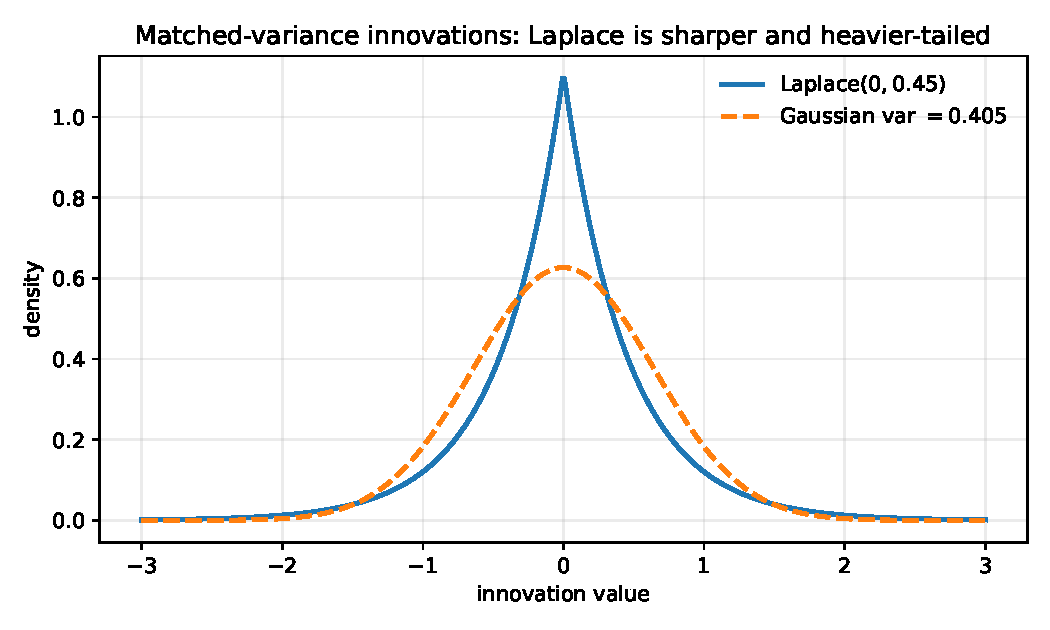
\includegraphics[width=.7\textwidth]{figures/fig01_innovation_compare.pdf}
\caption{Matched-variance innovations. The Laplace innovation has a sharper peak at zero and heavier tails than the Gaussian innovation with the same variance $2b^2$. The two models agree at second order but not beyond.}
\end{figure}

\begin{figure}[ht!]
\centering
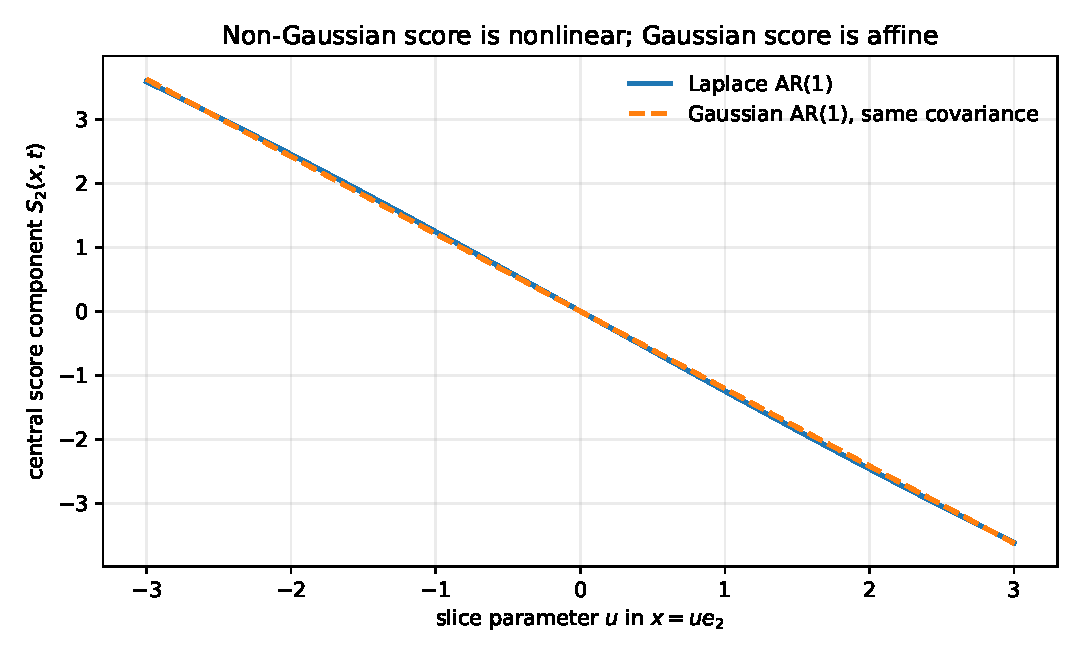
\includegraphics[width=.78\textwidth]{figures/fig02_score_slice.pdf}
\caption{A one-dimensional score slice for the noisy model. The Gaussian comparator with the same covariance gives a straight line because its score is affine. The Laplace score is visibly nonlinear.}
\end{figure}

\begin{figure}[ht!]
\centering
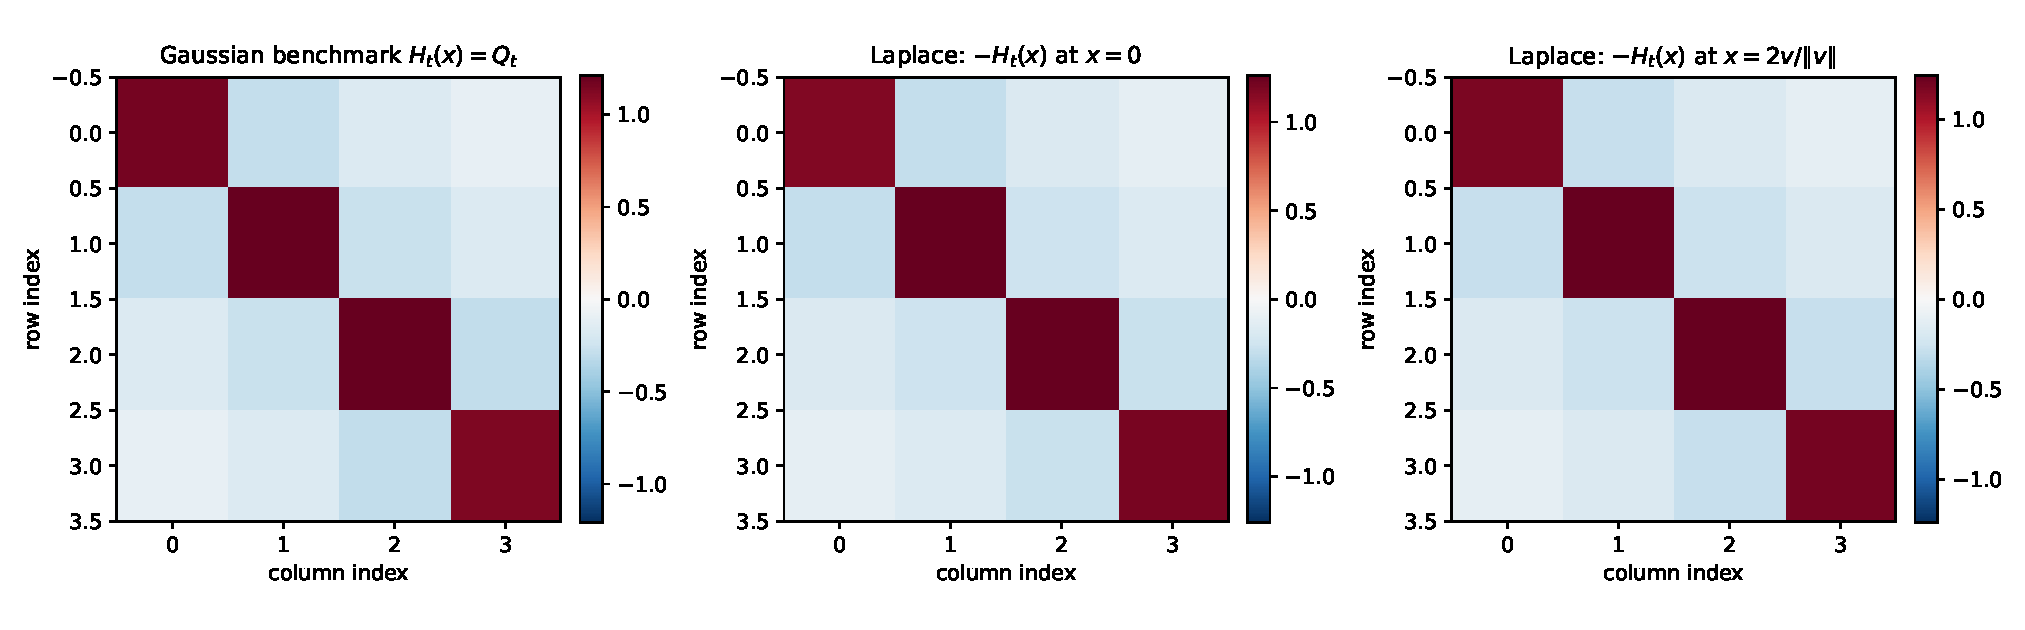
\includegraphics[width=.98\textwidth]{figures/fig03_hessian_heatmaps.pdf}
\caption{Generalized interaction matrices. In the Gaussian benchmark the negative log-density Hessian is the constant precision $Q_t$. In the Laplace model the corresponding matrix $H_t(x)$ depends on the location $x$. The two Laplace panels show that the interaction pattern changes across state space.}
\end{figure}

\begin{figure}[ht!]
\centering
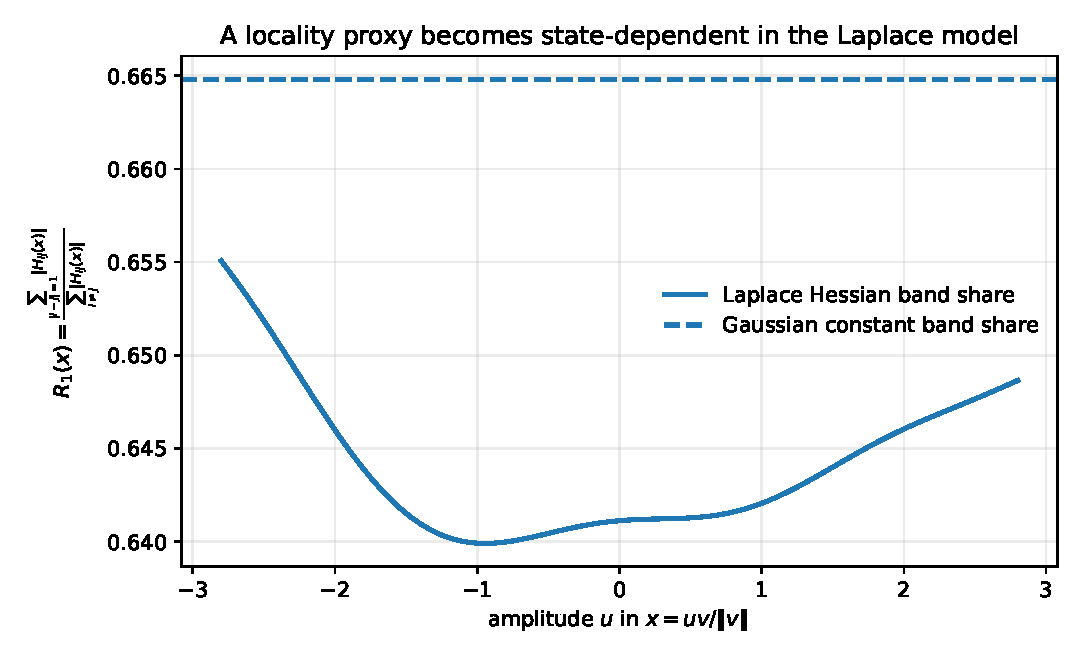
\includegraphics[width=.78\textwidth]{figures/fig04_hessian_bandshare.pdf}
\caption{State-dependent locality proxy. The Gaussian benchmark has a single constant nearest-neighbor band share. In the Laplace model the same quantity varies with the observation $x$, so locality is no longer summarized by one fixed matrix.}
\end{figure}

The numerical picture matches the derivations:
\begin{enumerate}[leftmargin=1.5em]
\item The score is nonlinear even after diffusion.
\item Matching the covariance to a Gaussian AR(1) model does not match the score.
\item The negative score Hessian is the right non-Gaussian analogue of a precision matrix, but it depends on $x$.
\item A notion of locality can survive only through observables like $R_r(x,t)$, not through exact zeros of a constant matrix.
\end{enumerate}

\section{Takeaway}
The Laplace AR(1) model separates the roles of Gaussianity and Markovianity cleanly.
\begin{itemize}[leftmargin=1.5em]
\item \textbf{Markovianity survives in the clean law.} The factorization \eqref{eq:clean_density} is nearest-neighbor and exact.
\item \textbf{Gaussianity is what is lost.} The characteristic function keeps quartic and higher terms at every finite time, so the noisy law is non-Gaussian and the score is nonlinear.
\item \textbf{Precision is replaced by a field of Hessians.} The matrix $H_t(x)$ in \eqref{eq:H_cov} is the natural generalized interaction object. It reduces to the usual precision only in the Gaussian case.
\end{itemize}

So the conceptual decomposition is:
\[
\text{Gaussianity} \Rightarrow \text{affine score and constant Hessian},
\]
\[
\text{Markovianity} \Rightarrow \text{local clean factorization},
\]
\[
\text{non-Gaussian diffusion} \Rightarrow \text{state-dependent interactions }H_t(x).
\]
This is precisely what breaks when we move beyond the Gaussian benchmark.

\end{document}
